
\chapter{Optimization of the Selection} \label{Optimization of Selection}
In chapter three, the selection of the analysis are presented, and $\Delta \eta$, mass of AK8 jet, and working points of double-b tagger have been optimized. The procedure will be introduced in the chapter.

\section{$\Delta \eta$}
The selection of $\Delta \eta$ is mainly to reject the multi-jet events. Tje optimization is done through changing the value of $\Delta \eta$ selection and picking up the one whose Punzi significance, $\frac{\varepsilon _{signal}}{1+\sqrt{N_{bkg}}}$, is the highest, where $\varepsilon _{signal}$ is the efficiency of the signal and $N_{bkg}$ is the the number of events of background (MC multi-jet events). Through the difference of different is little, the value of 1.1 or 1.2 is favored in low mass region, while larger values are suited for higher mass region. However, the $\Delta \eta$ will change the trigger turn-on curve. Hence, we decided to use 1.3 for all mass region for both signal samples.

\begin{figure}[t]
  \centering
  \begin{tabular}{cc}
    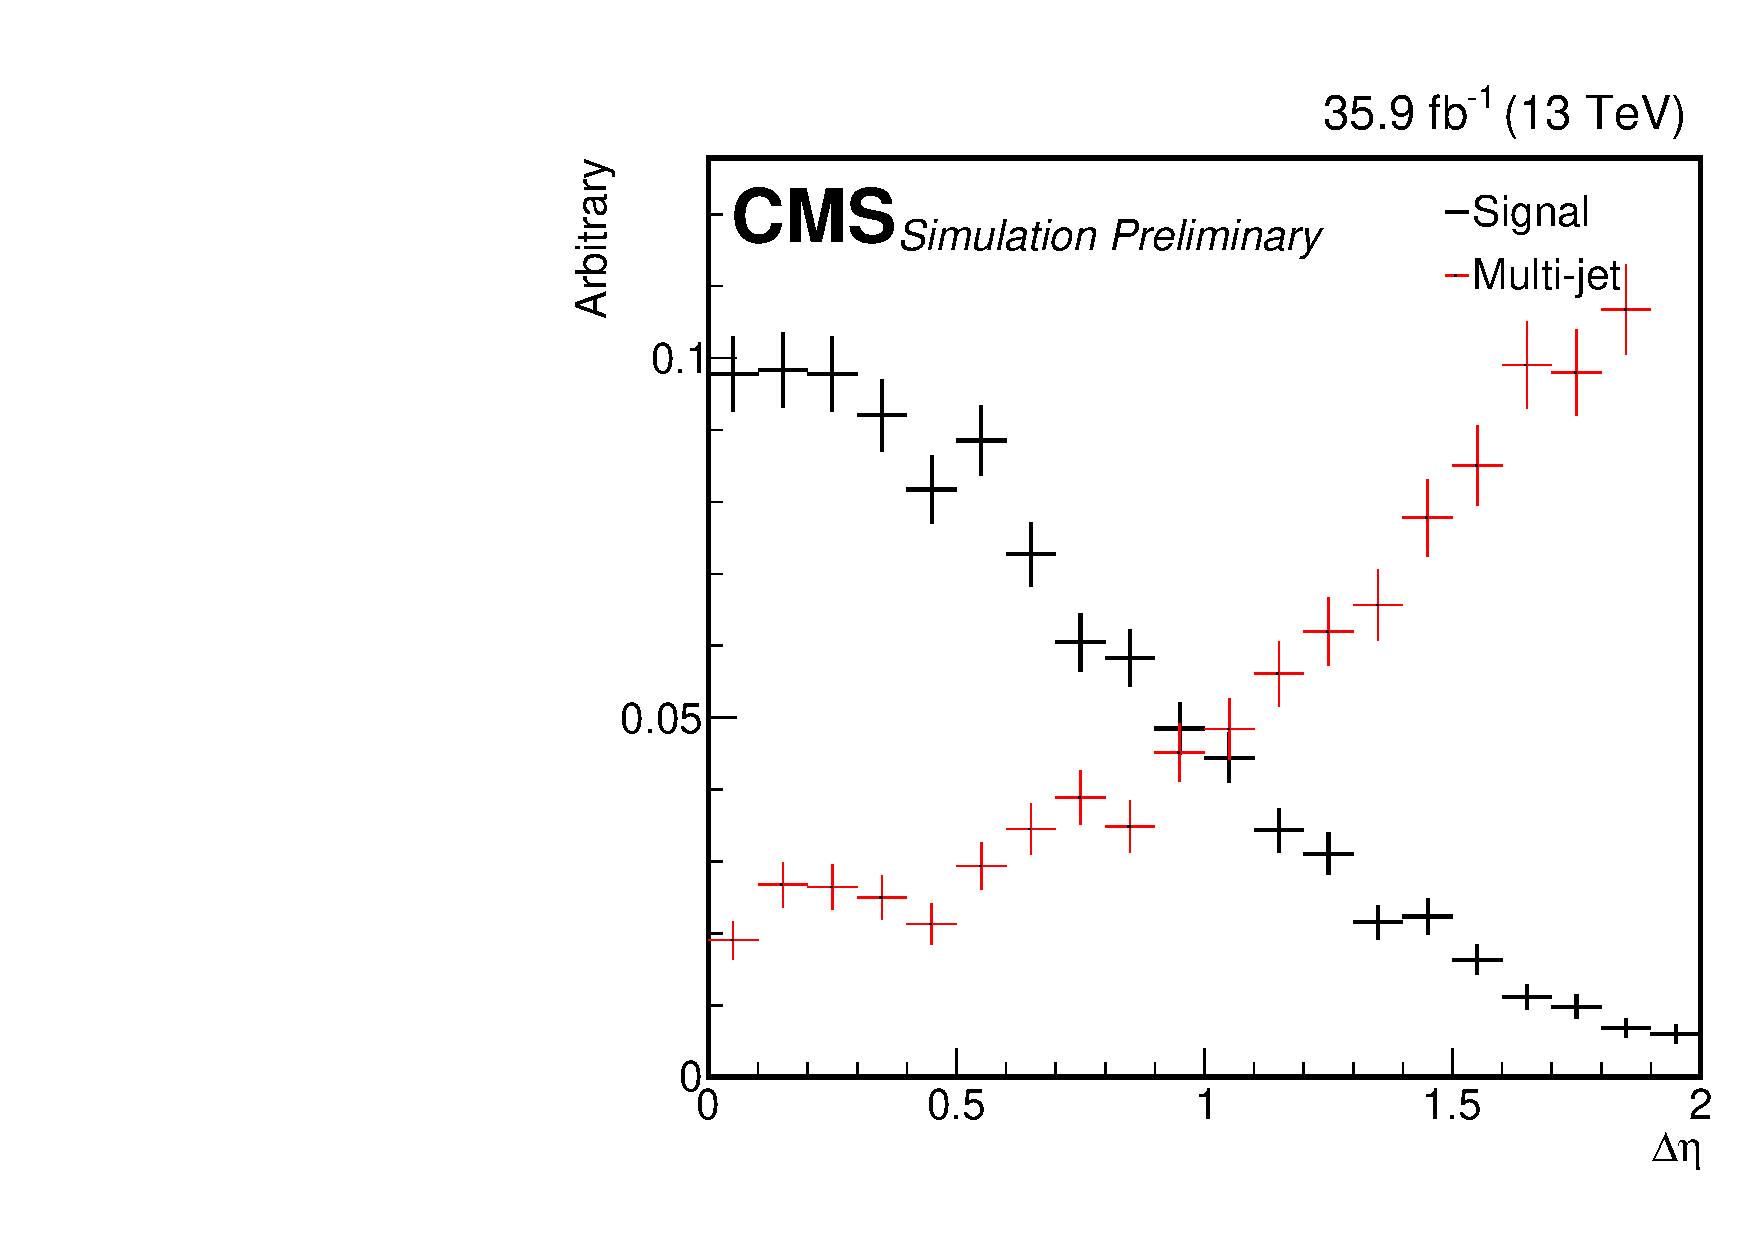
\includegraphics[width=0.5\textwidth]{Figures/deta/bulk/TT1400.pdf} &
       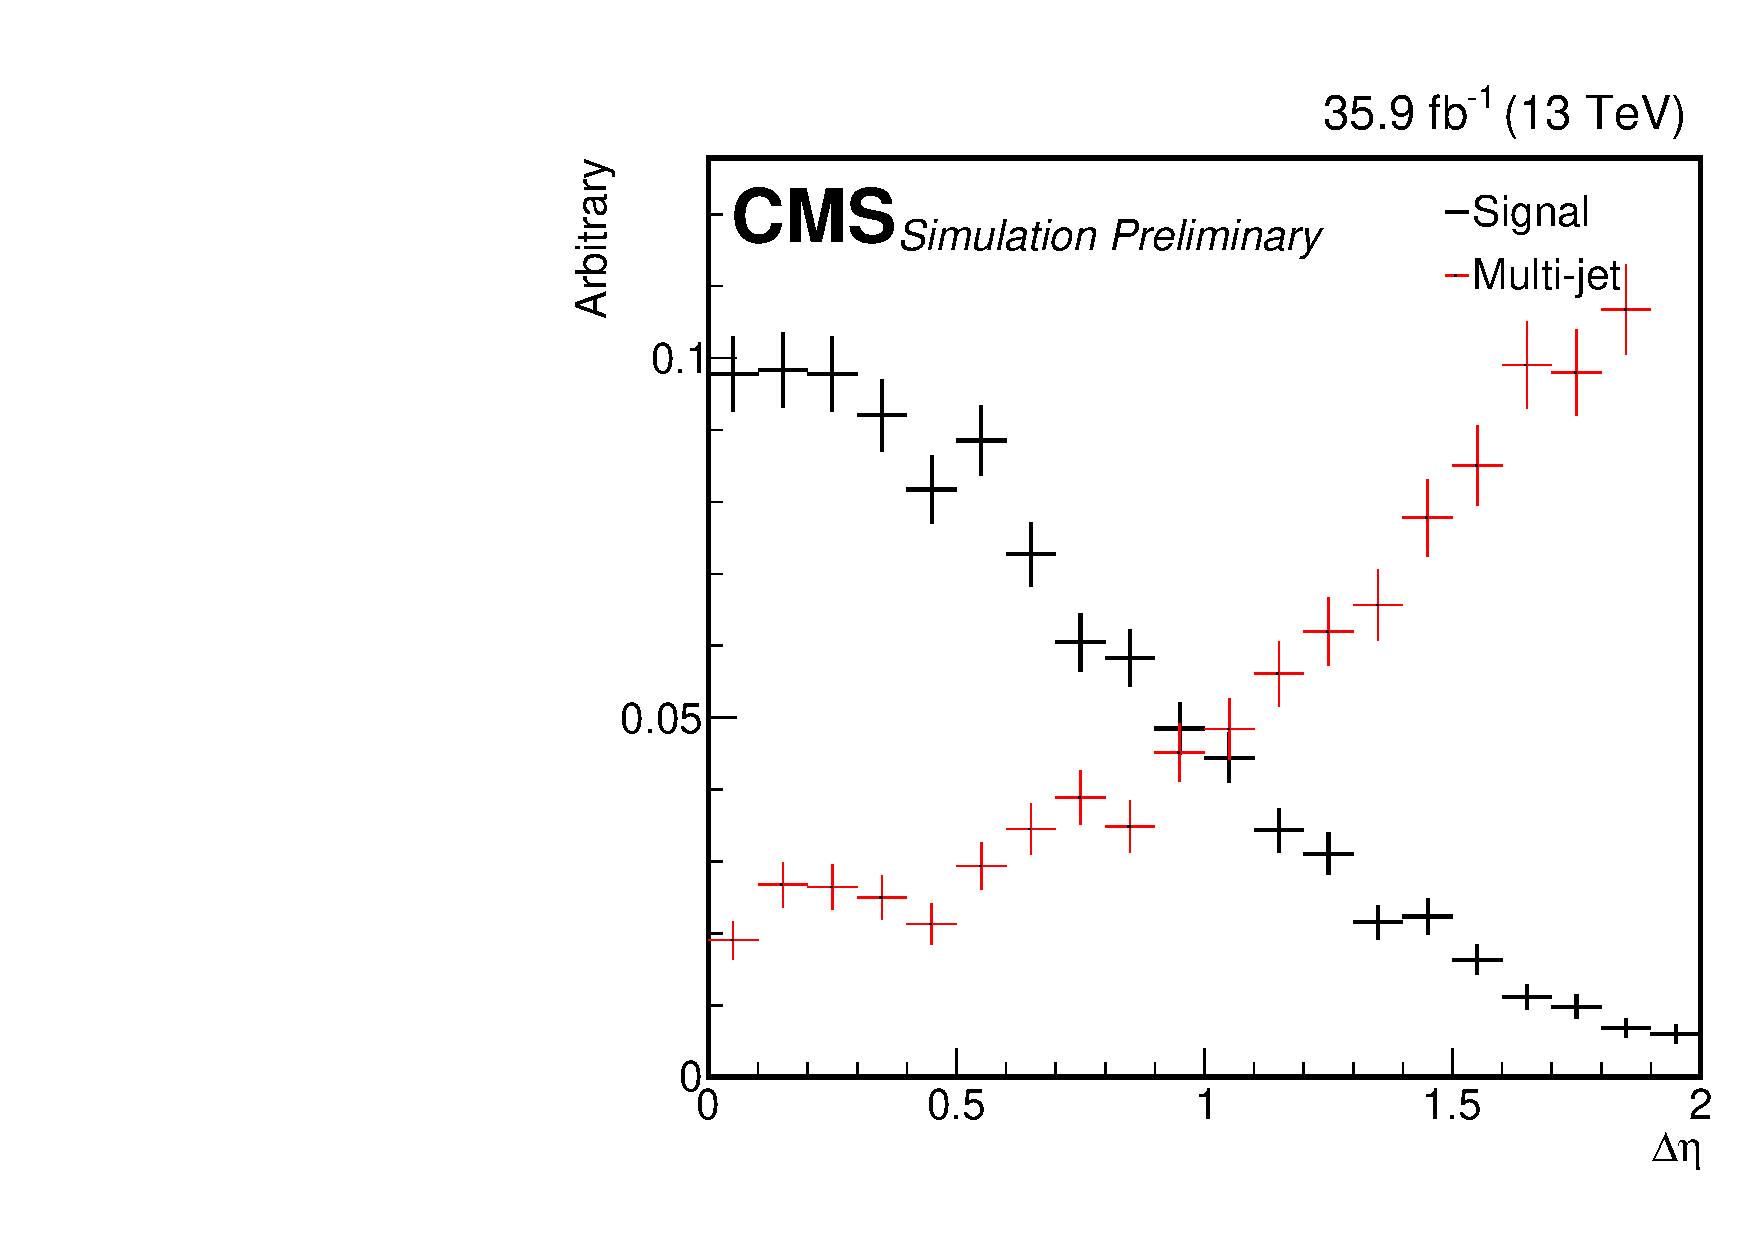
\includegraphics[width=0.5\textwidth]{Figures/deta/bulk/TT1400.pdf}
  \end{tabular}
  \caption{The distribution of $\Delta \eta$ of 1.4 TeV bulk graviton and of multi-jet in TT (left) and LL (right) category.}

\end{figure}

\begin{figure}[t]
  \centering
  \begin{tabular}{cc}
    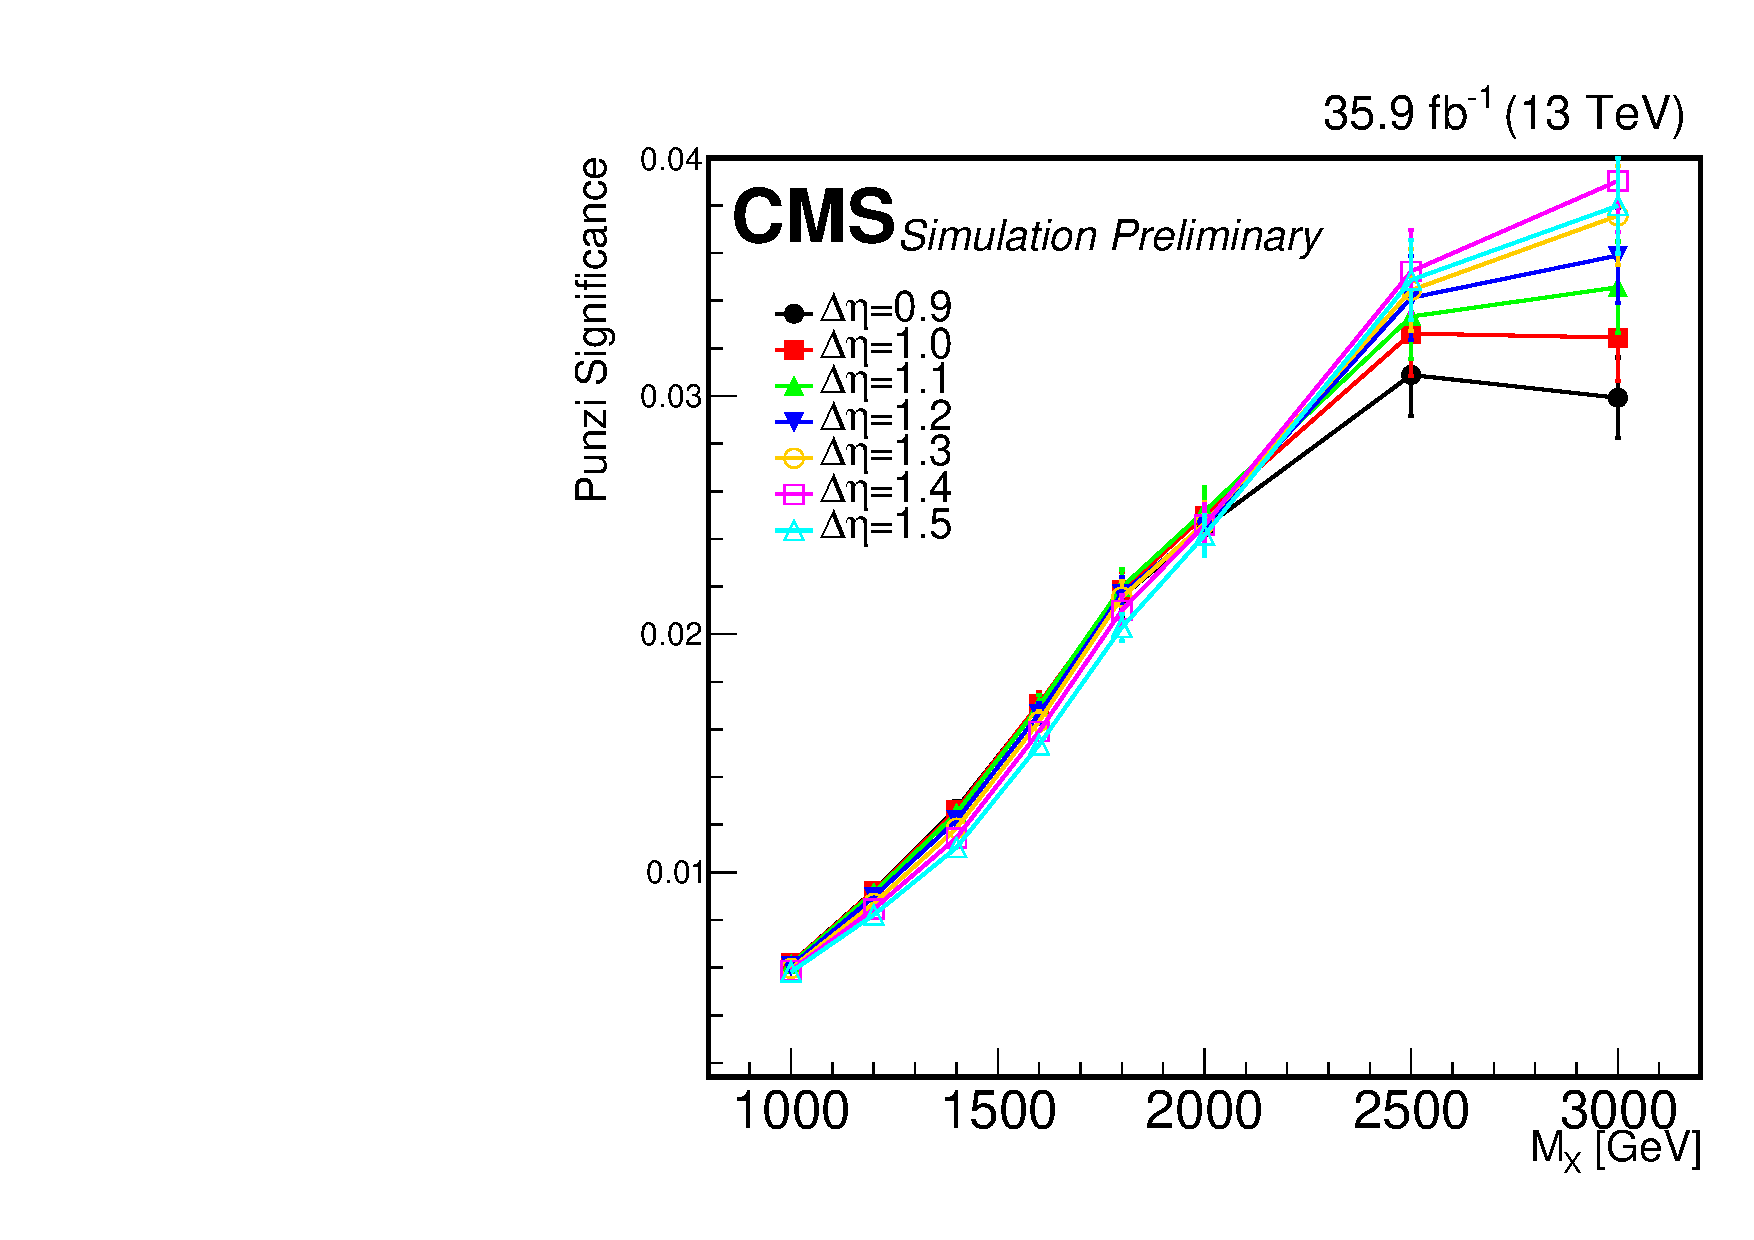
\includegraphics[width=0.5\textwidth]{Figures/deta/bulk/dEtaTT.pdf} &
       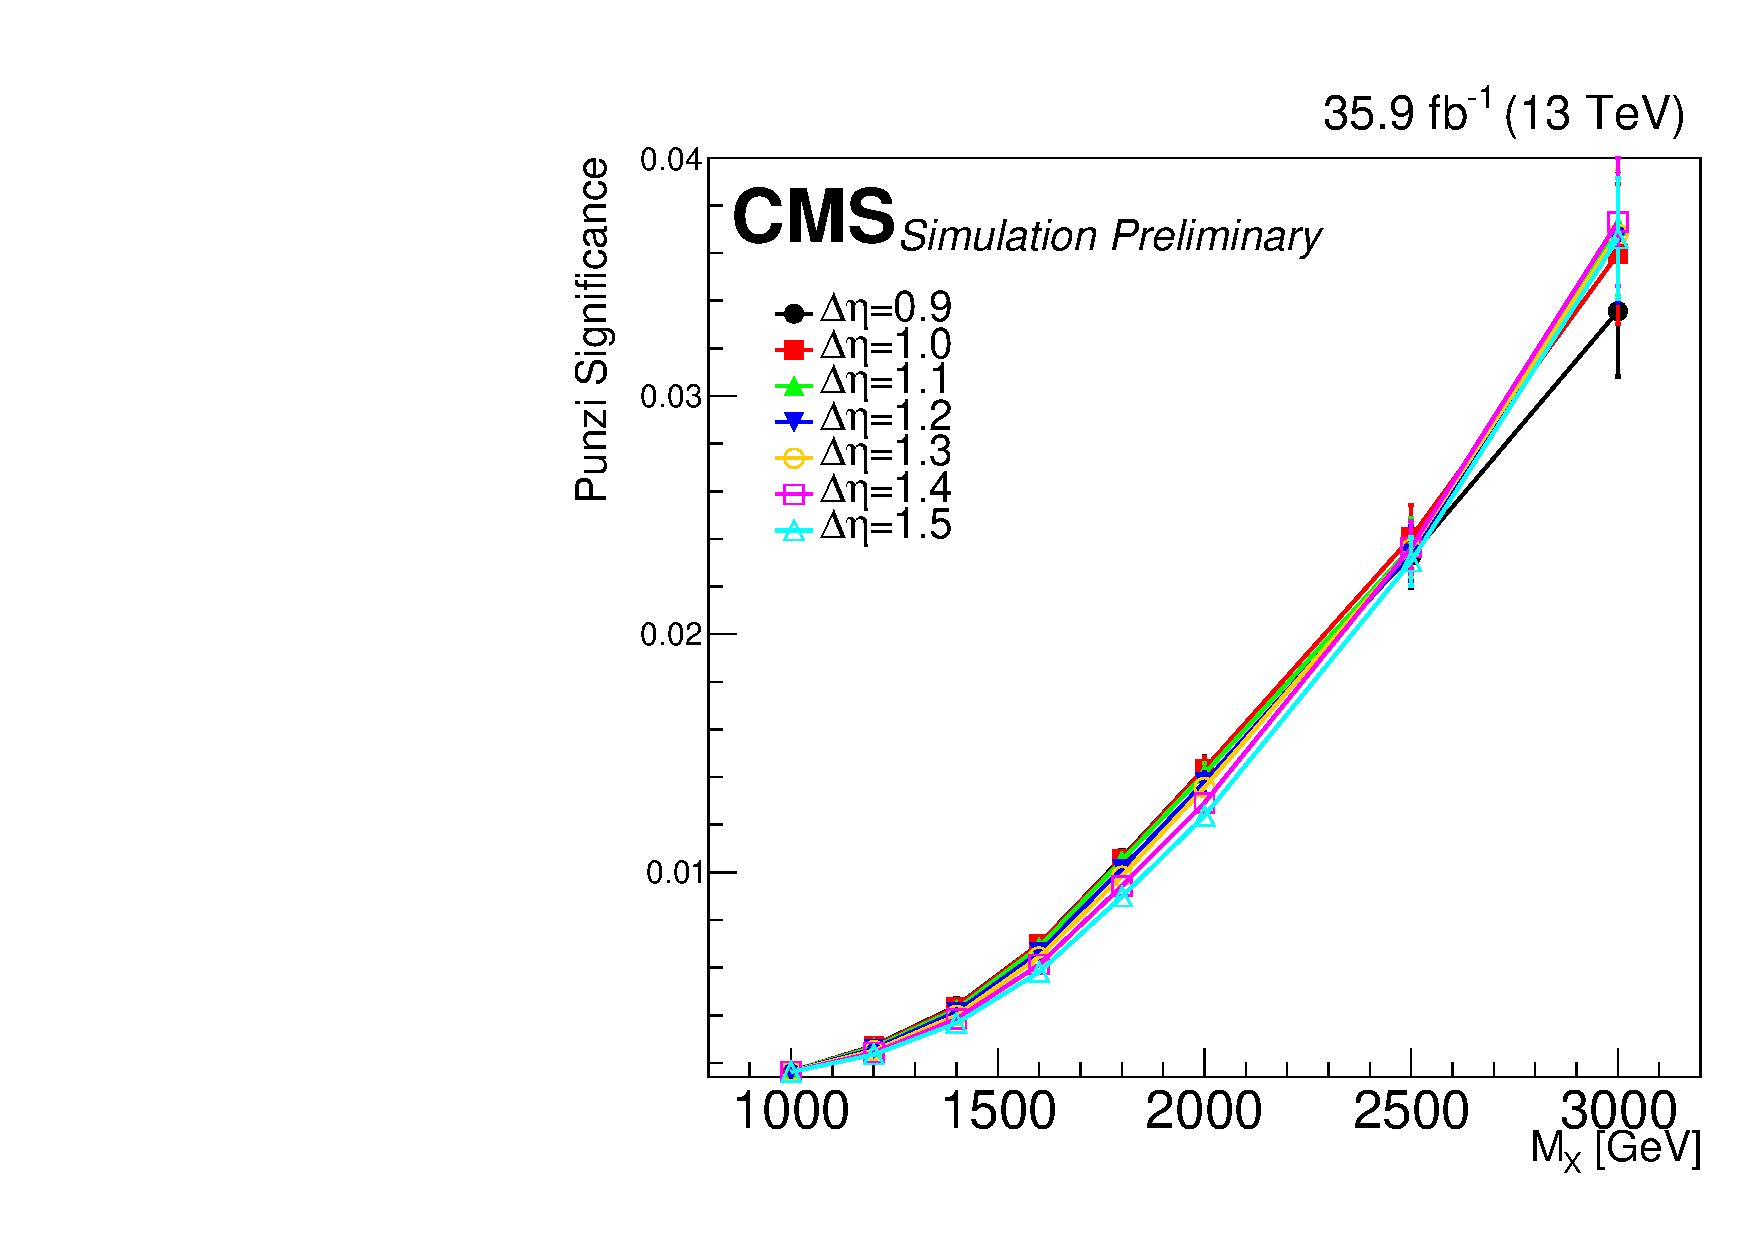
\includegraphics[width=0.5\textwidth]{Figures/deta/bulk/dEtaLL.pdf}
  \end{tabular}
  \caption{The Punzi significance of different cut value of $\Delta \eta$ in TT (left) and LL (right) category of bulk graviton.}

\end{figure}

\begin{figure}[t]
  \centering
  \begin{tabular}{cc}
    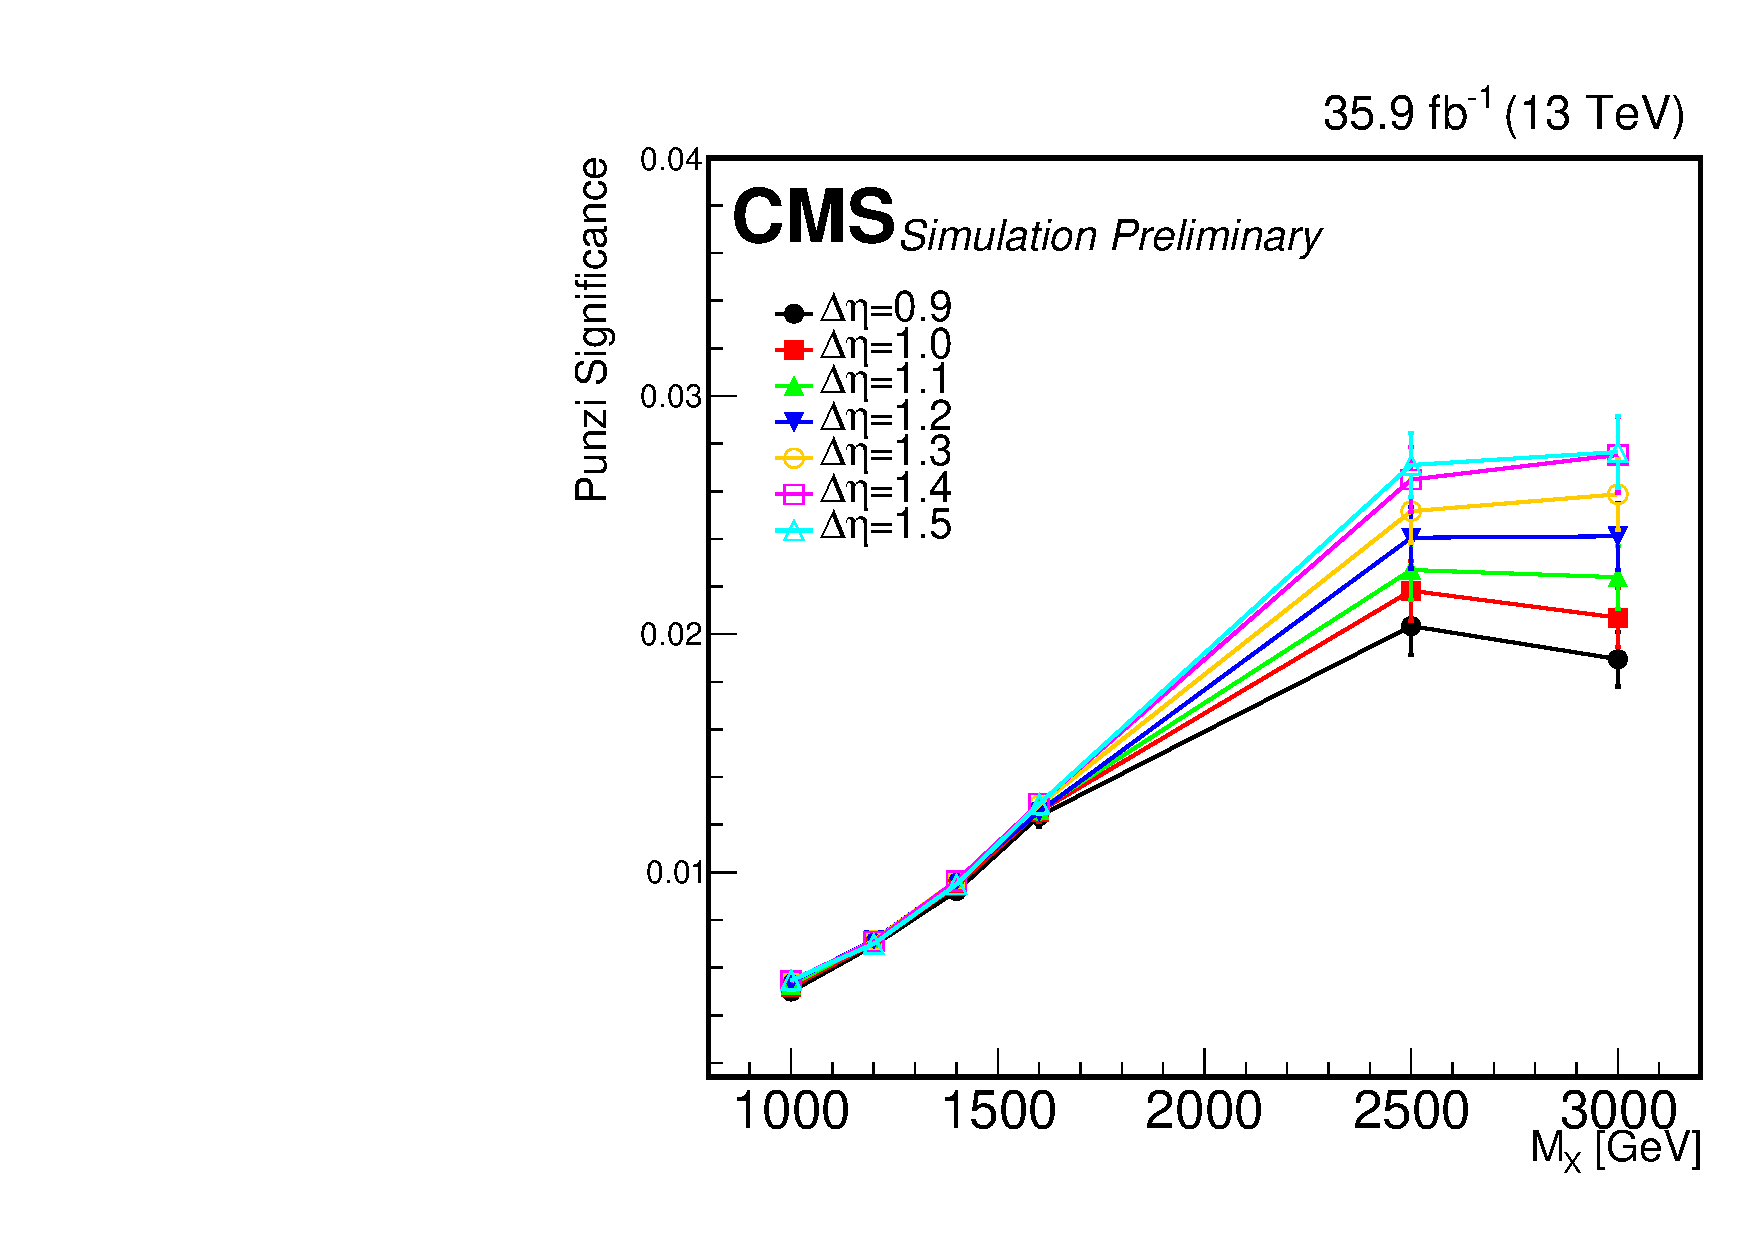
\includegraphics[width=0.5\textwidth]{Figures/deta/rad/dEtaTT.pdf} &
       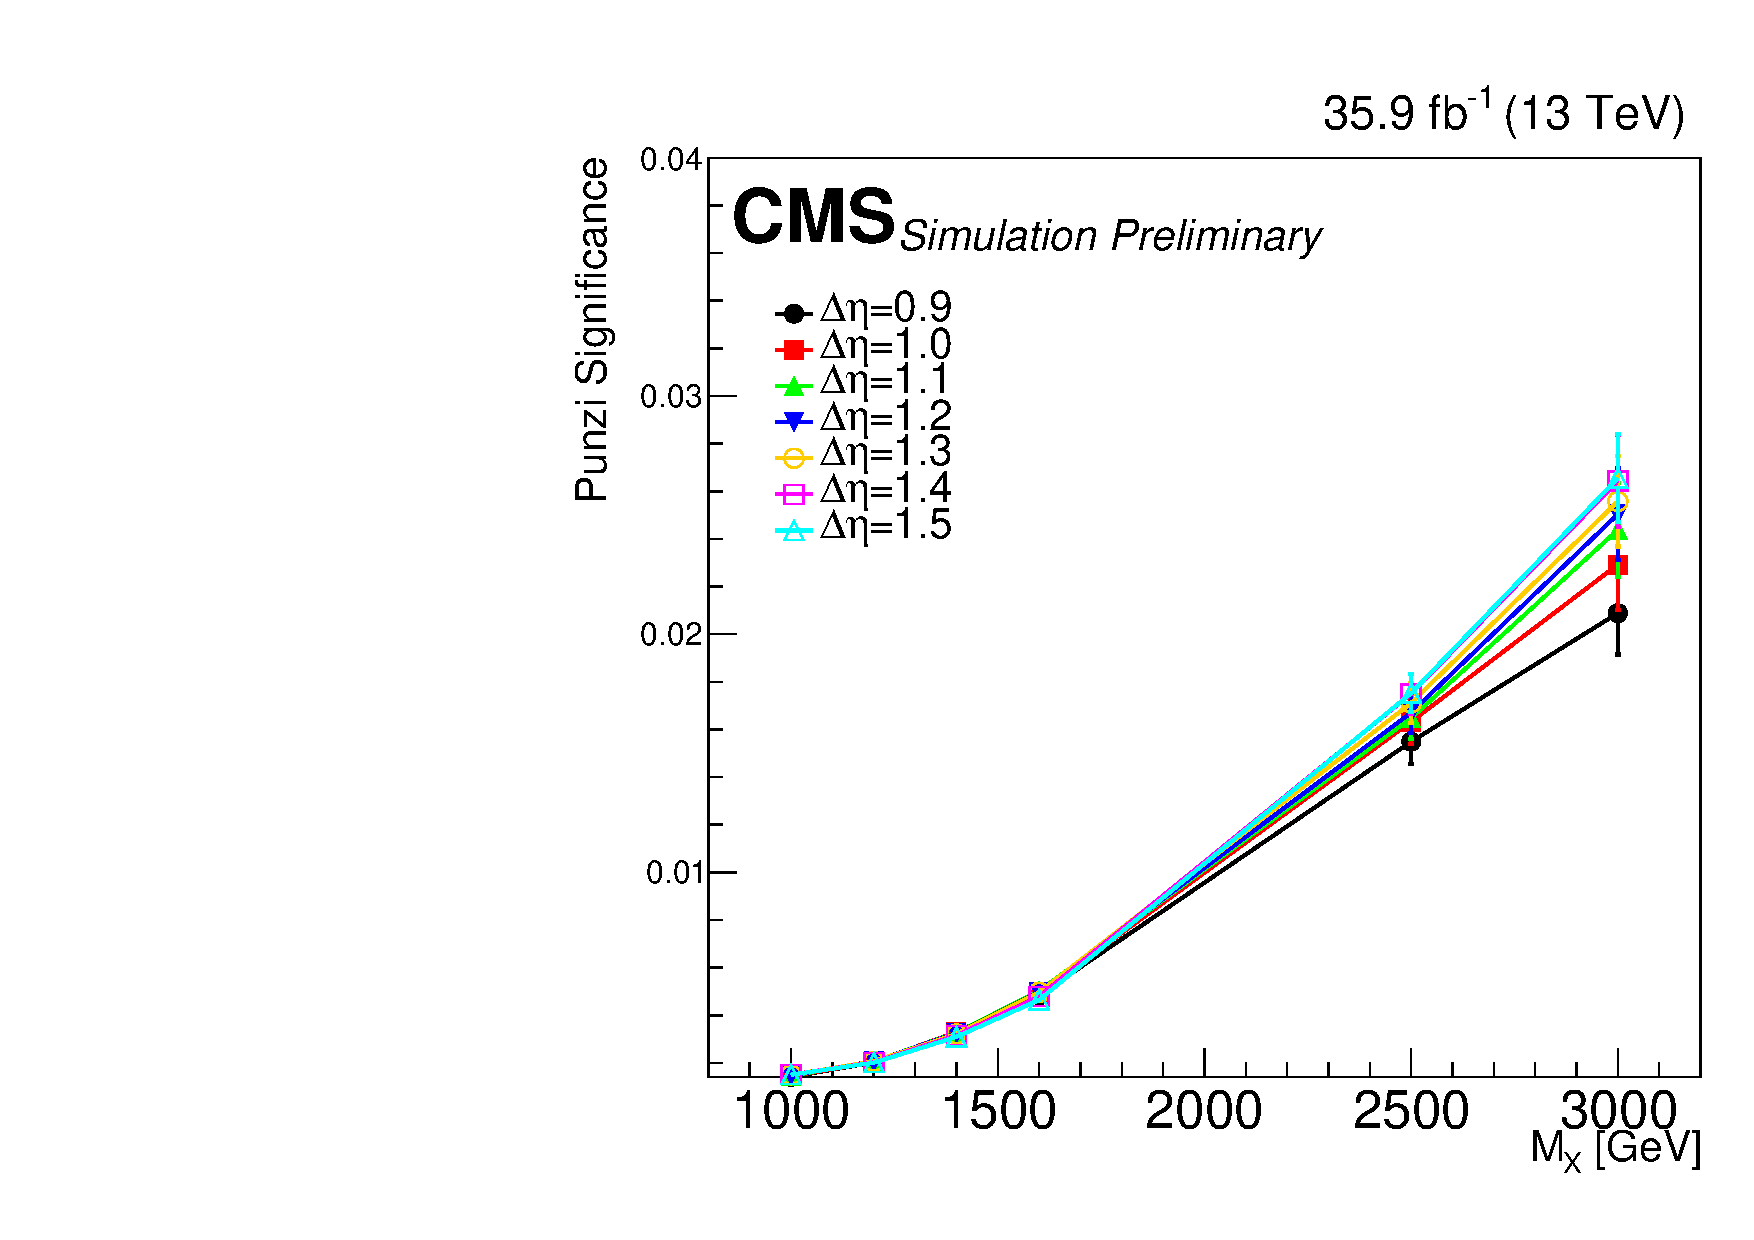
\includegraphics[width=0.5\textwidth]{Figures/deta/rad/dEtaLL.pdf}
  \end{tabular}
  \caption{The Punzi significance of different cut value of $\Delta \eta$ in TT (left) and LL (right) category of radion.}

\end{figure}

\clearpage
\section{Double-b Tagger}
There are two AK8 jets in an events of the analysis. Each AK8 jet corresponds to a working point of double-b tagger, either tight ($>$0.8), medium ($>$0.6), or loose ($>$0.3). The combinations are: 
\begin{itemize}
\item TT: two passing tight.
\item TM: one passing tight, the other passing medium.
\item TL: one passing tight, the other passing loose.
\item MM: two passing medium.
\item ML: one passing medium, the other passing loose.
\item LL: two passing loose.
\end{itemize}
The optimization is based on 95 $\% $ upper limit on $\sigma$(pp $\rightarrow$ X $\rightarrow$ HH) $\times$ Br(HH $\rightarrow$ $b\bar{b}b\bar{b}$) by bump hunt background estimation. The TT region gives the best limit. Therefore, we further combine TT category with other categories to see if there is any improvement. Noted that the result is compared with 2015 analysis using another algorithm of b tagger, sub-jet b tagger, in three of four sub-jets in two AK8 jets passing selection and in four of them passing selection, which are referred as 3b and 4b respectively. We consider these combinations where each category is excluded from TT category:

\begin{itemize}
\item TM+TT
\item TL+TT
\item MM+TT
\item ML+TT
\item LL+TT
\end{itemize}
The TT combined with LL gives the best limit.

\begin{figure}[t]
  \centering
  \begin{tabular}{cc}
    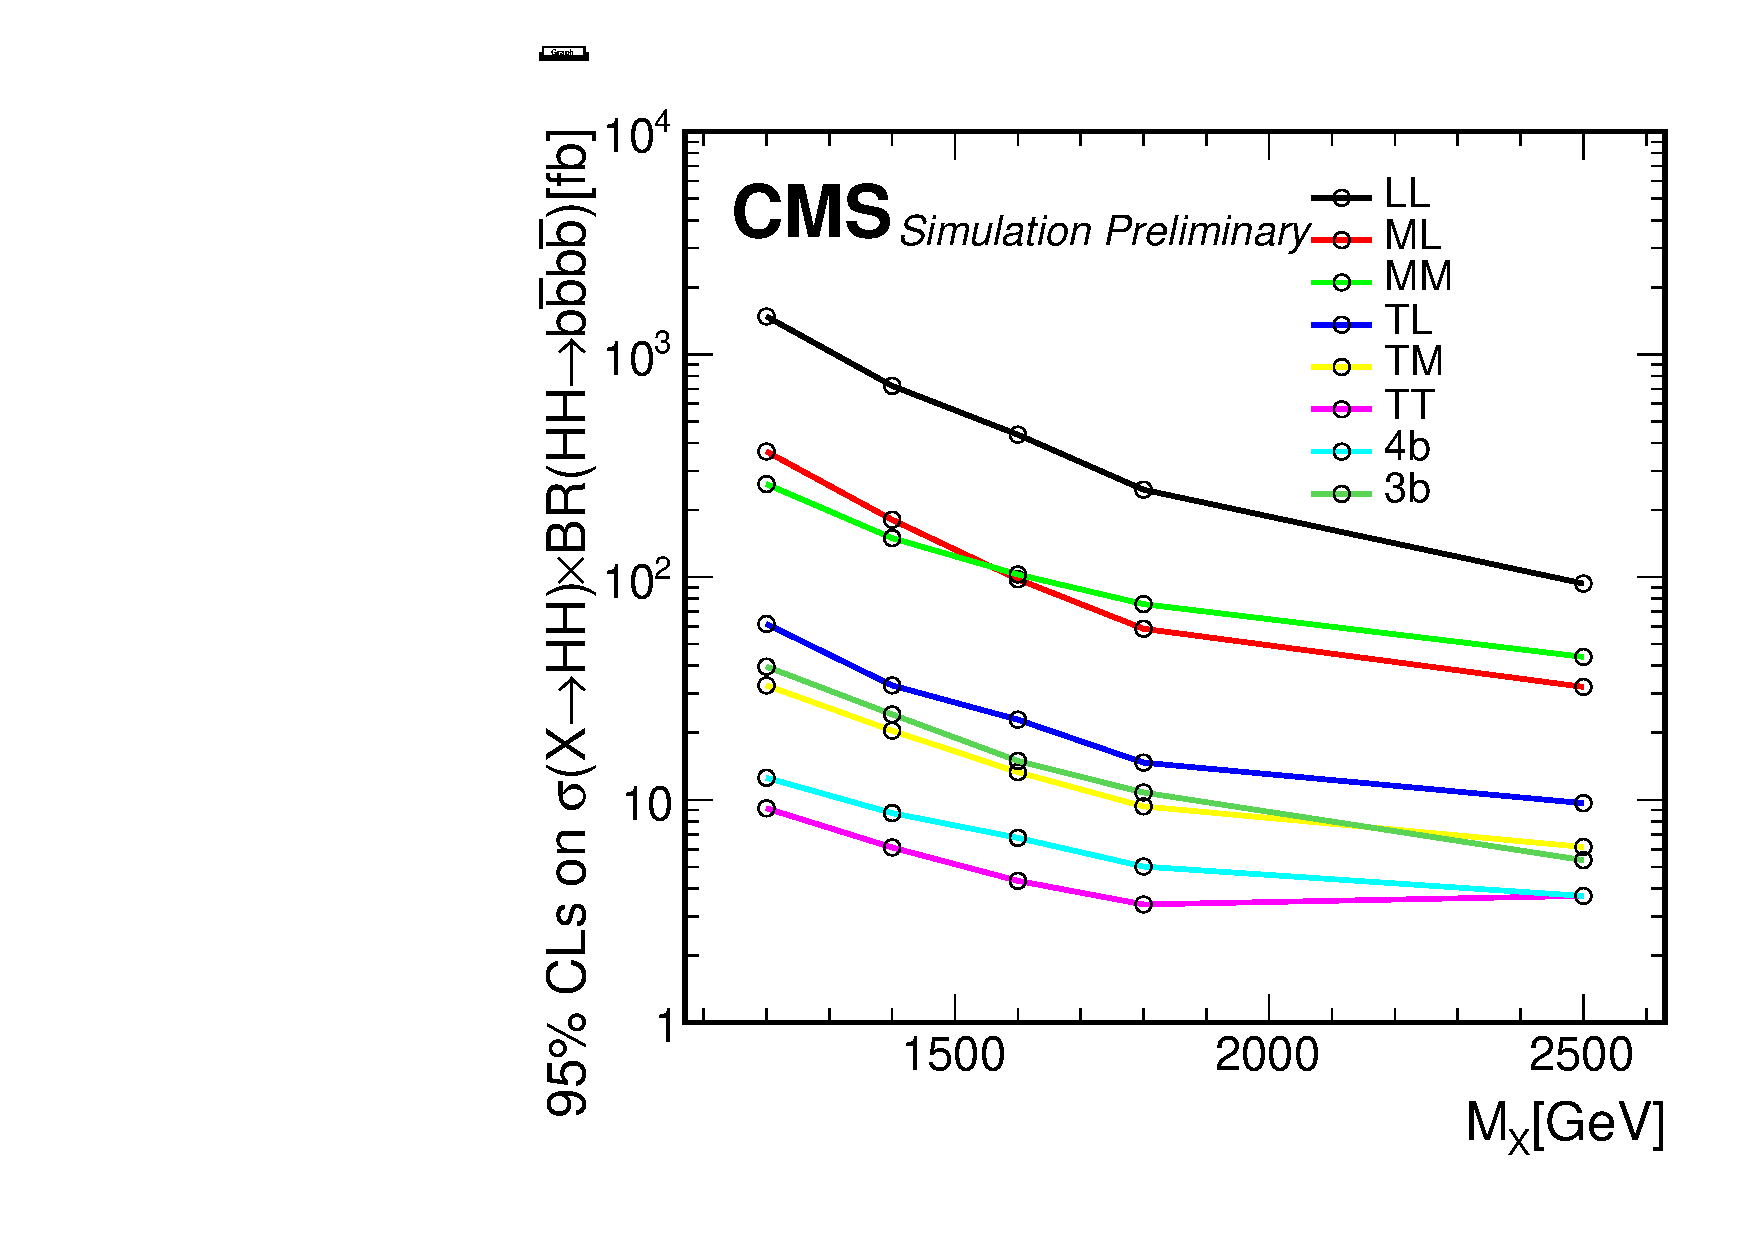
\includegraphics[width=0.5\textwidth]{Figures/BDTLimit.pdf} &
    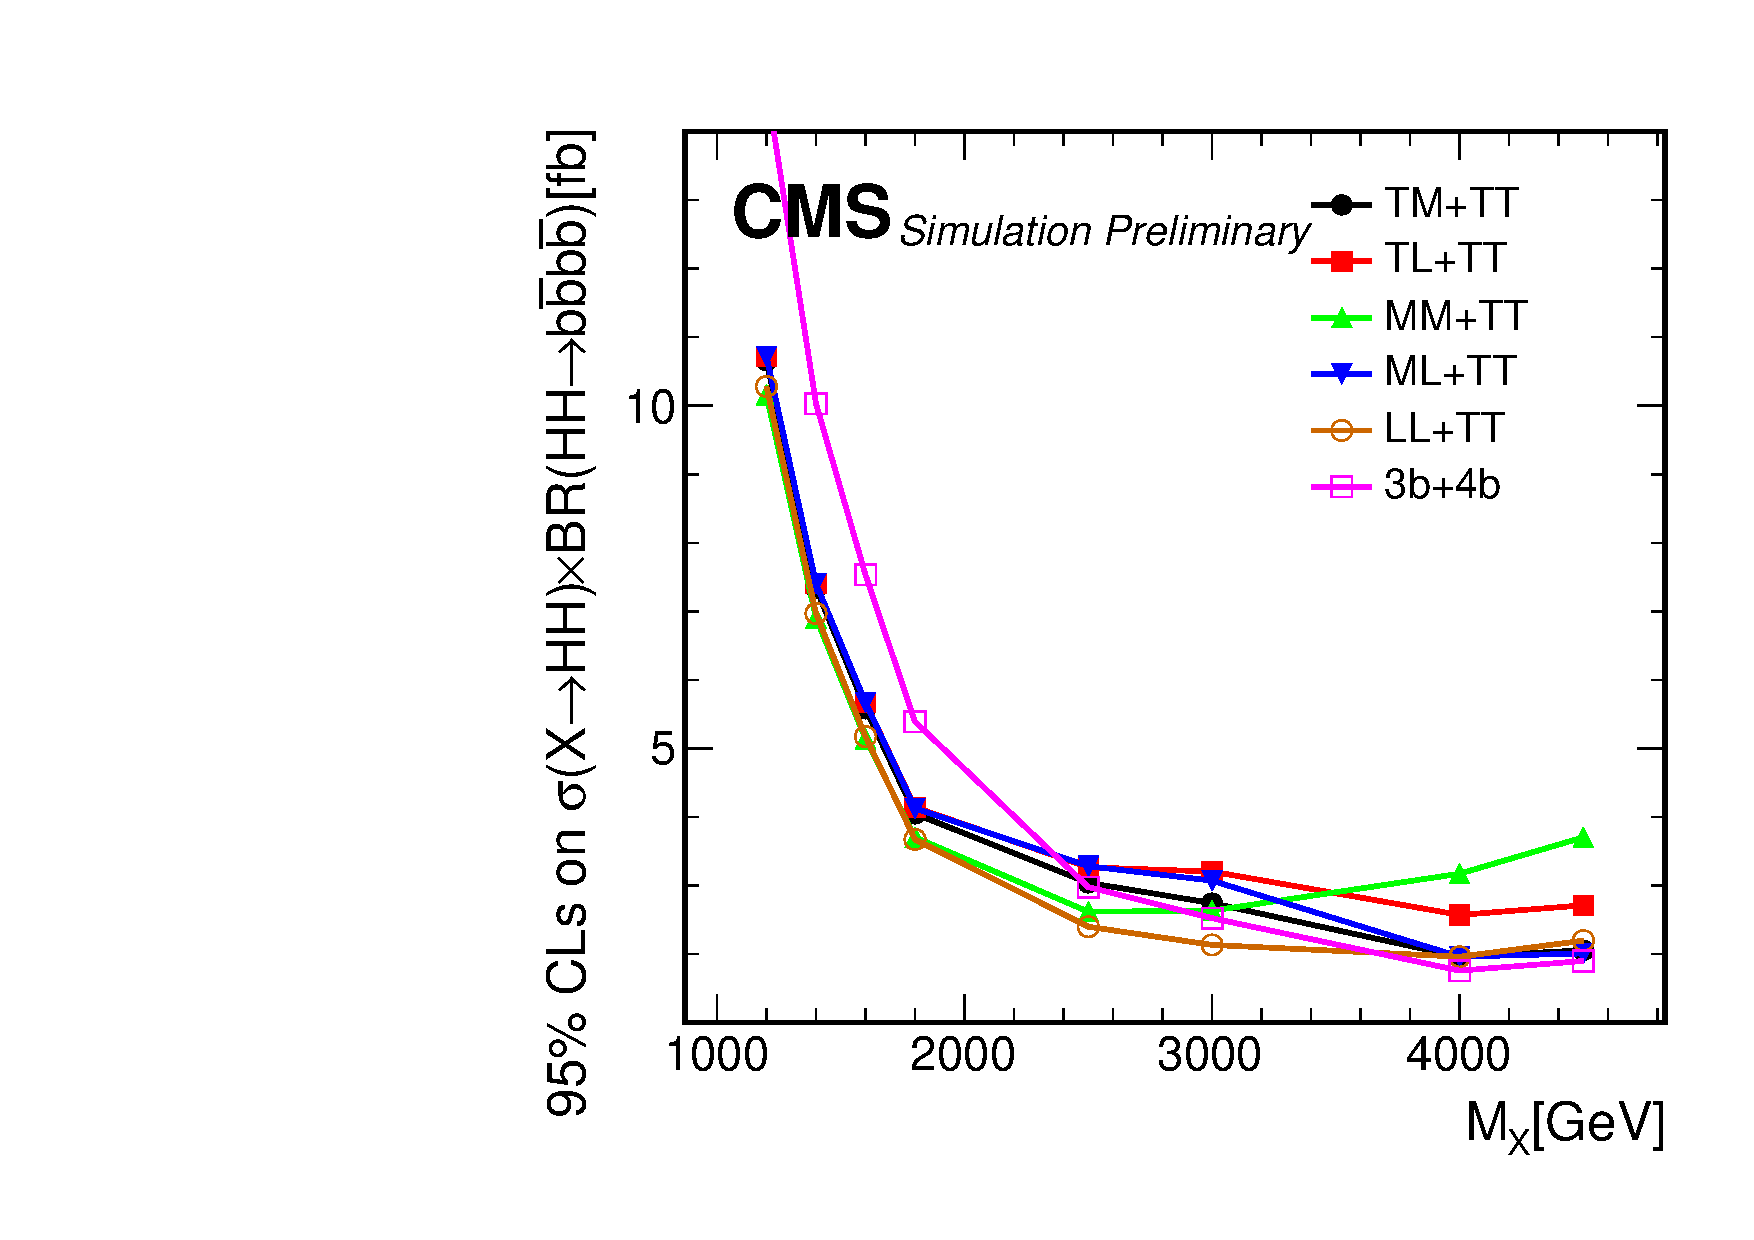
\includegraphics[width=0.5\textwidth]{Figures/BDTLimitcombine.pdf}
  \end{tabular}
  \caption{The 95$\% $ upper limit on $\sigma$(pp $\rightarrow$ X $\rightarrow$ HH) $\times$ Br(HH $\rightarrow$ $b\bar{b}b\bar{b}$) with different double-b tagger category.}

\end{figure}

\clearpage
\section{Mass of AK8 Jet}
In order to tag the AK8 jet as Higgs jet, the selection around mass of Higgs boson is required, while the range should not cover the mass of Z boson and top quark. The width of the windows from 25 to 40 GeV is considered. All mass windows used are listed. Besides the PUPPI soft-drop mass with the W boson correction, the one with the Higgs dedicated correction is also targeted. The Higgs dedicated correction is done using similar procedure of the W boson correction. The samples are X $\rightarrow$ HH rather than X $\rightarrow$ WW. In addition, the Higgs dedicated correction uses one-step correction, which correction the mass of reconstruction-level to the mass of physical Higgs boson, while the W boson correction corrects first to generator-level then to the mass of physical Higgs boson. Both of them remove the dependence of the mass on jet p$_{T}$. The optimization is done based on 95 $\% $ upper limit on $\sigma$(pp $\rightarrow$ X $\rightarrow$ HH) $\times$ Br(HH $\rightarrow$ $b\bar{b}b\bar{b}$) by alphabet background estimation. The result shows that the mass with Higgs boson correction gives better limit of less than 10 $\% $.

\begin{table}[h!]
  \begin{center}
   \begin{tabular}{|l|l|l|l|l|}
\hline
\multirow{2}{*}{Lower Range (GeV)} & \multicolumn{4}{l|}{Width (GeV)} \\ \cline{2-5} 
                                   & 25     & 30     & 35     & 40    \\ \hline
100                                & 100-125 & 100-130  &  100-135  &  100-140     \\ \hline
105      &  105-130      &   105-135     &  105-140      &    105-145   \\ \hline
110      &  110-135      &   110-140     &  110-145      &    not considered   \\ \hline
115      &  115-140      &   115-145     &  not considered      &    not considered   \\ \hline
\end{tabular}
\caption{The mass windows used for optimization.}
  \end{center}
  \end{table}


\begin{figure}[t]
  \centering
  \begin{tabular}{c}
    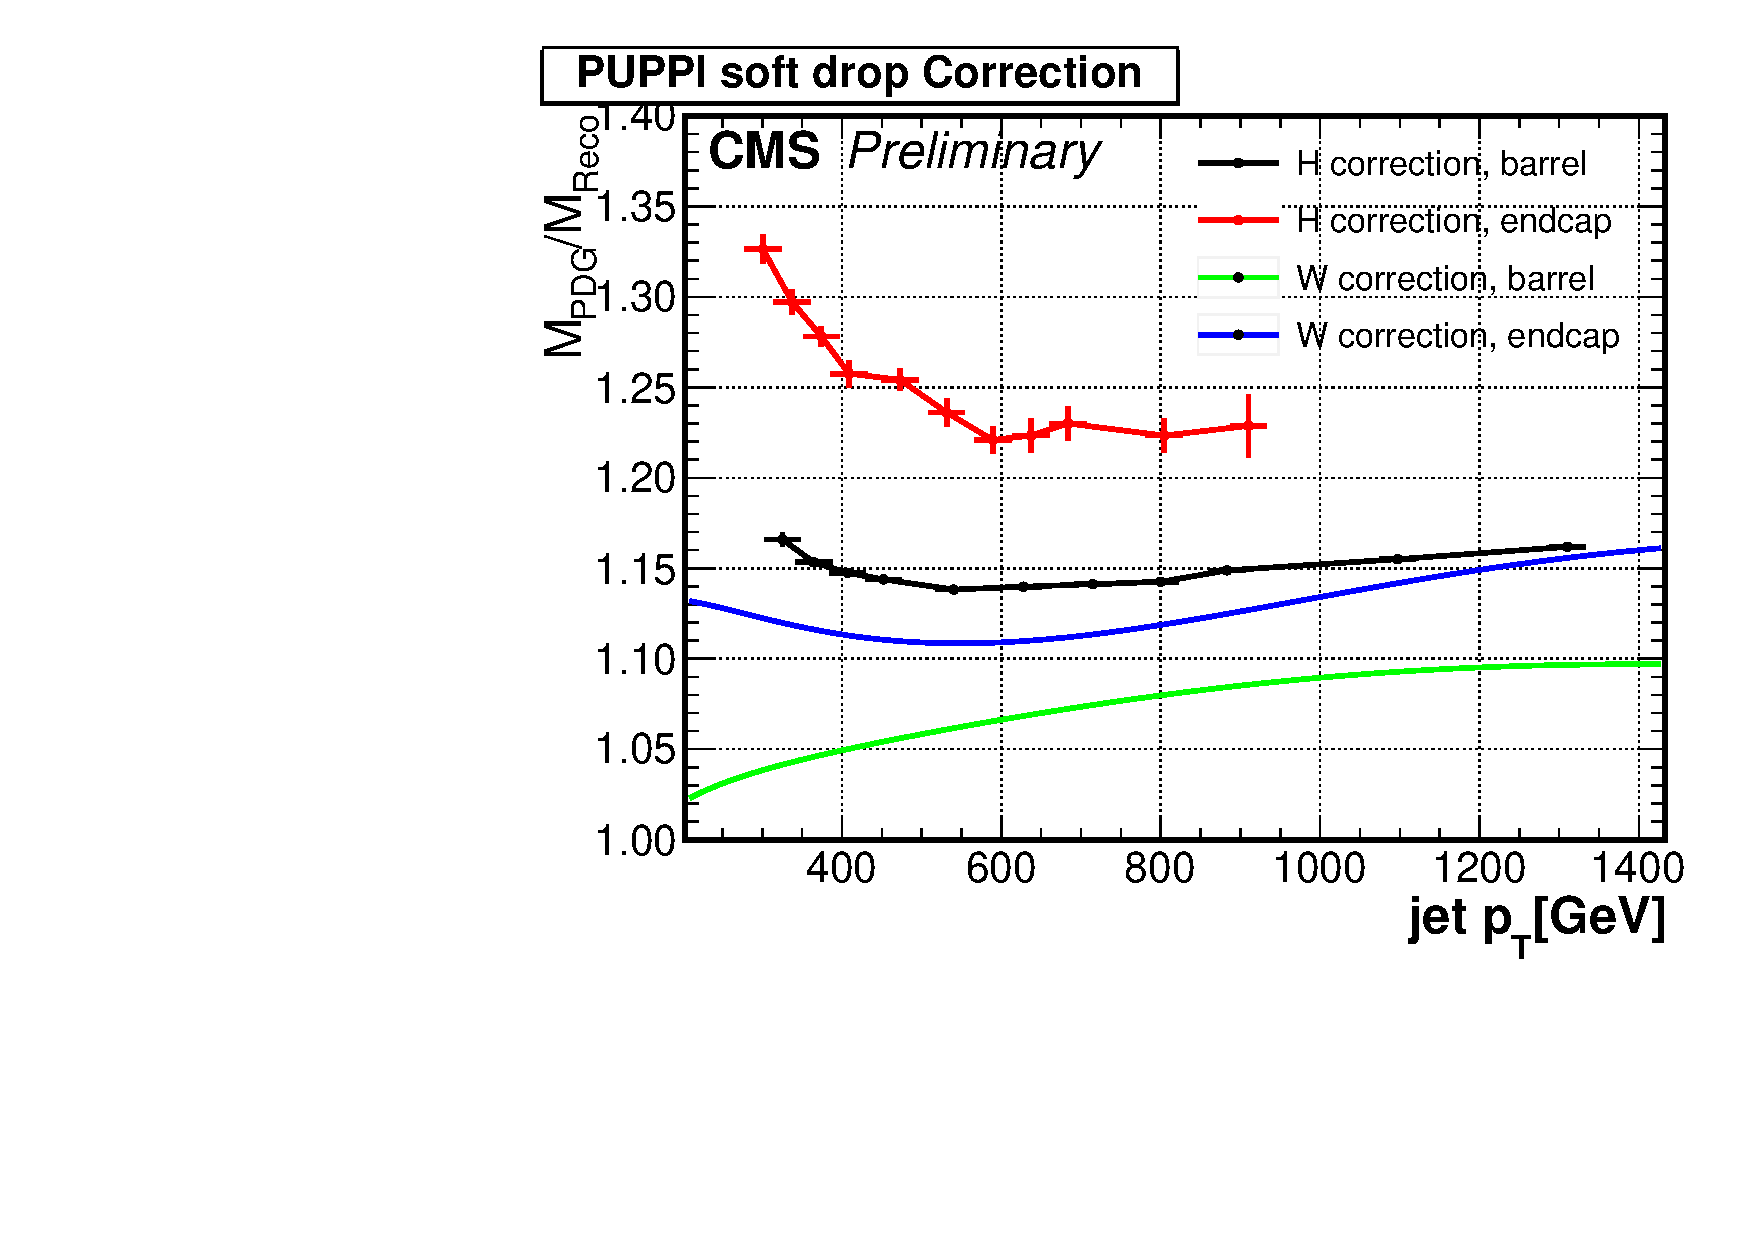
\includegraphics[width=0.5\textwidth]{Figures/ap1/recoOne.pdf} 
  \end{tabular}
  \caption{The weights versus jet p$_{T}$ of W boson and of Higgs boson correction.}

\end{figure}

\begin{figure}[t]
  \centering
  \begin{tabular}{cc}
    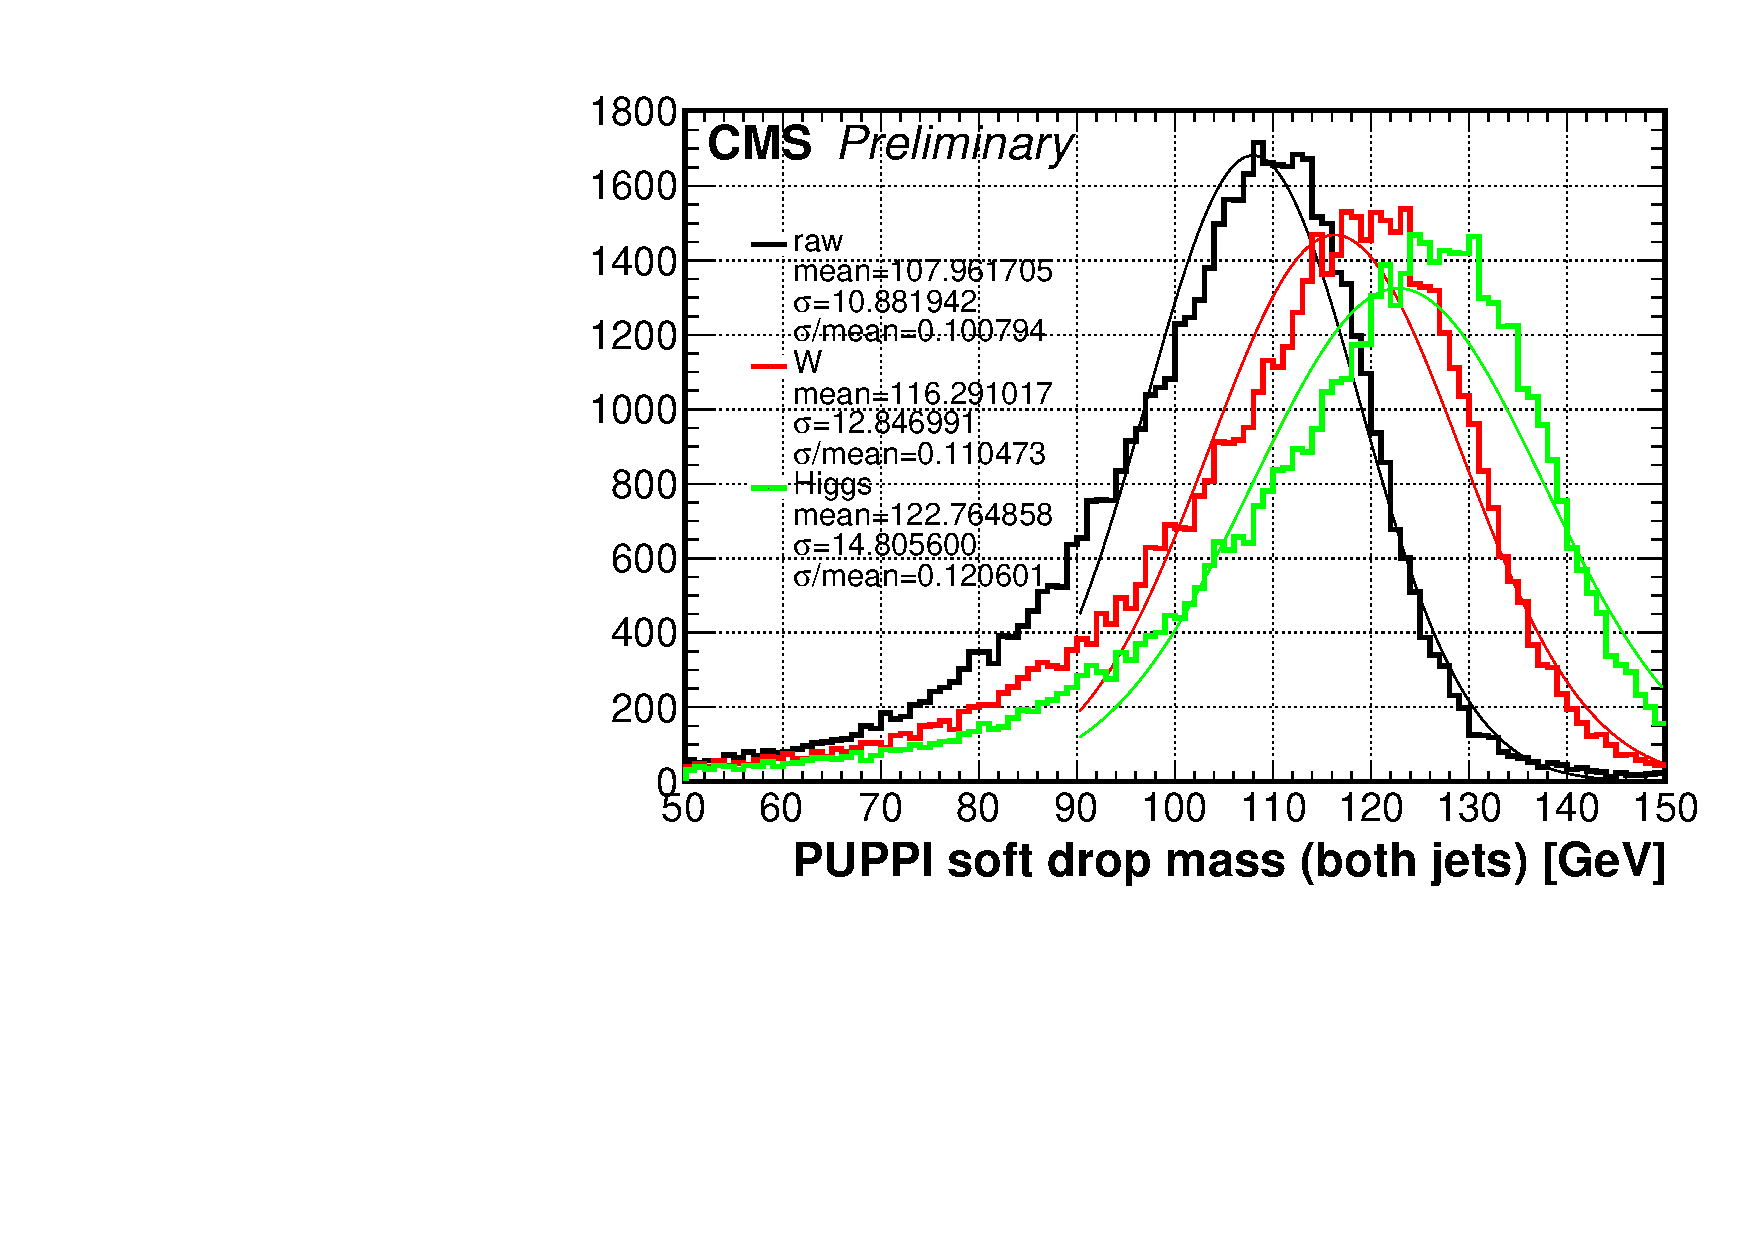
\includegraphics[width=0.5\textwidth]{Figures/ap1/j01.pdf}  &
    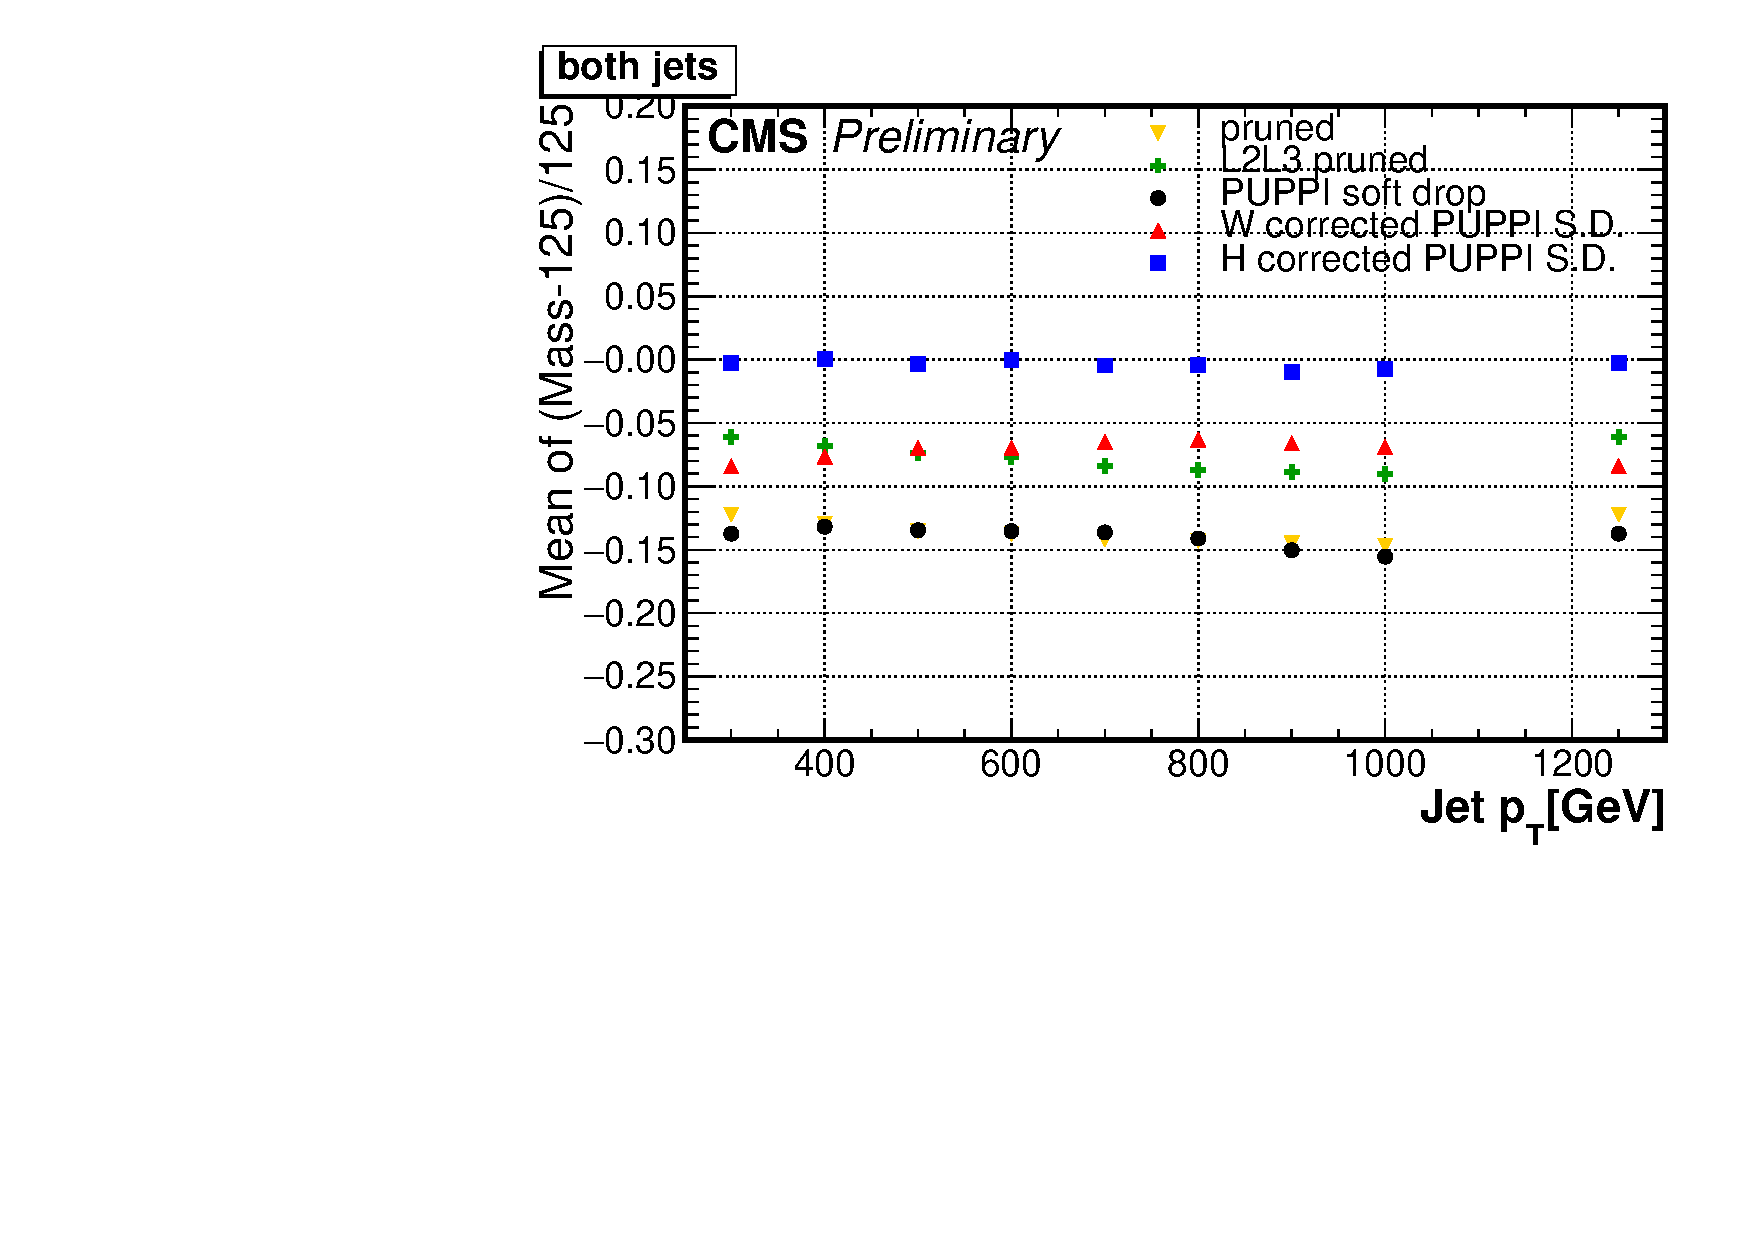
\includegraphics[width=0.5\textwidth]{Figures/ap1/MassMean_both.pdf} \\
  \end{tabular}
  \caption{The corrected PUPPI soft-drop mass (left) filled with leading and next leading AK8 jets and the mean of the Gaussian fit on the mass of versus the jet p$_{T}$ (right). One point on the curve corresponds to one mass point of signal.}

\end{figure}

\begin{figure}[t]
  \centering
  \begin{tabular}{c}
    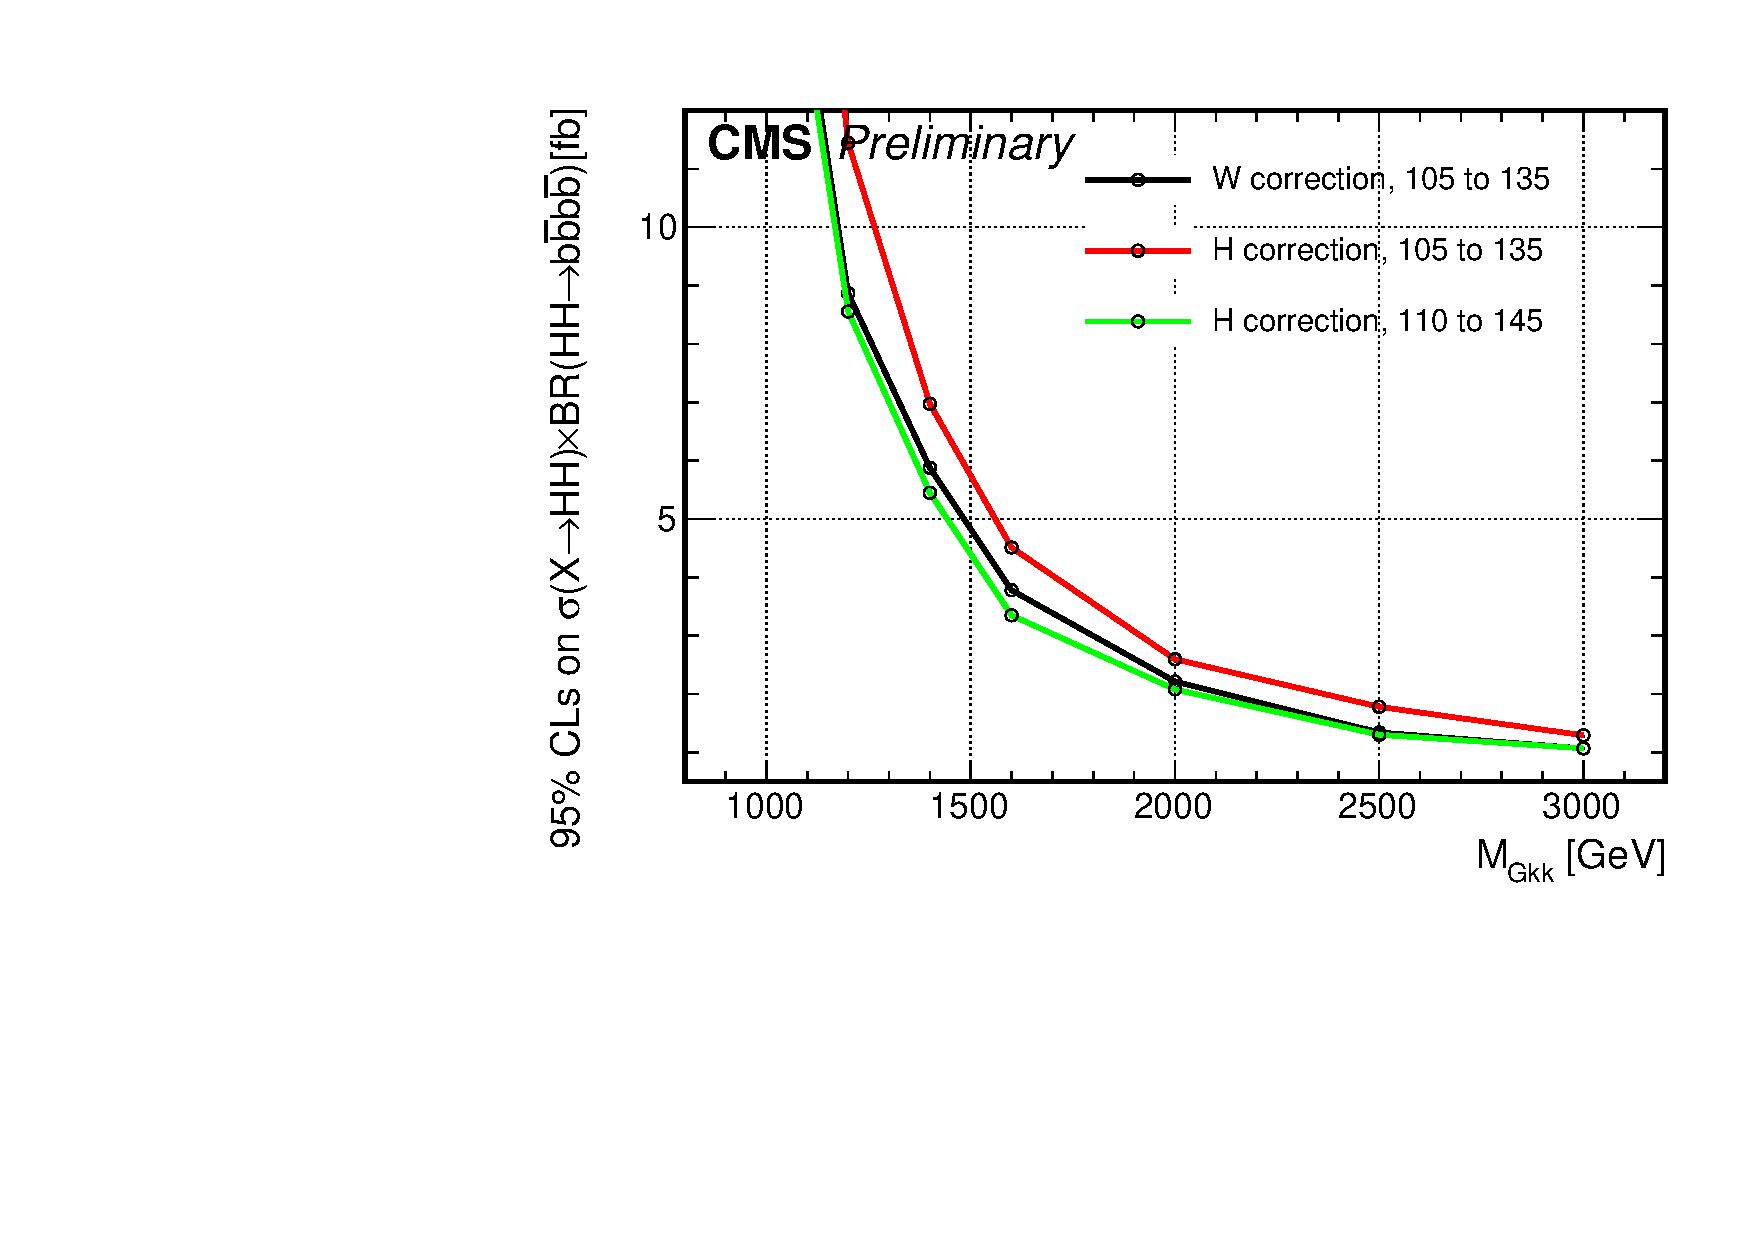
\includegraphics[width=0.5\textwidth]{Figures/ap1/Limit2.pdf} 
  \end{tabular}
  \caption{The 95$\% $ upper limit on $\sigma$(pp $\rightarrow$ X $\rightarrow$ HH) $\times$ Br(HH $\rightarrow$ $b\bar{b}b\bar{b}$) with different mass windows of different mass correction.}

\end{figure}
